\section{Pure-Shift Spectra via \acl{2DJ} Estimation}
\label{sec:pure-shift}

Two key features of the \ac{NMR} experiment for which improvements are
constantly being sought are sensitivity and resolving power. There are numerous
means of enhancing sensitivity, including technological advancements such as
production of superconducting magnets with higher field
strengths\cite{Maeda2019} (sensitivity $\propto B_0^{\nicefrac{7}{4}}$) and
cryogenic probes\cite{Styles1984,Styles1989,Kovacs2005}, as well as simply
increasing the number of scans (sensitivity $\propto \sqrt{\text{no. scans}}$).
However, few means of achieving better resolution exist beyond increased field
strengths (resolution $\propto B_0$). \note{Perhaps mention improved field
homogeneities (shimming)?} Significant interest has therefore been given to the
development of techniques which generate broadband homodecoupled (\emph{pure
shift}) spectra, in which the effects of homonuclear scalar couplings are
absent from the data. While often valuable for structural assignment purposes,
their influence can lead to spectra which are too crowded for meaningful
insights to be gleamed. Heteronuclear couplings are straightforward to decouple
at the point of \ac{FID} acquisition\cite{Shaka1983a, Shaka1983b,Shaka1985}.
The removal of homonuclear couplings associated with a specific spin can also
be achieved by irradiating said spin with a weak \ac{RF} field\cite[Section
4.2]{Claridge2016}. Broadband homodecoupling, in which all spins
are simultaneously decoupled from each other, is a more challenging task. At
the time of writing, there are a number of of well-established pure shift
experiments, which involve running a \ac{2D} pulse sequence, and concatenating
the initial section of each \ac{FID}. in a process referred to as
chunking\cite{Meyer2013,Adams2014,Zangger2015}. The key drawback of all of
these techniques is the hit to sensitivity, a result of the fact that a subset
\note{Does ``subset'' make sense?} of the available spin magnetisation
contributes to the signal. At the time of writing, the state-of-the-art
pure shift technique is arguably \ac{PSYCHE}, both because of its sensitivity,
and its ability to cope with strong couplings. \note{Describe strong couplings
if this has not been done before now}. In this section, a method for deriving
pure shift spectra indirectly via the estimation of \ac{2DJ} datasets is
presented, named \acf{CUPID}.

In this section, an overview of the key techniques which have
been developed to generate pure shift spectra is given, starting with \ac{2DJ}
spectroscopy and finishing up with \ac{PSYCHE}, widely considered the most
robust pure shift experiment in terms of sensitivity and tolerance to strong
coupling. Subsequently, a new technique for generating pure shift spectra via
parametric estimation, named \acf{CUPID} is presented.

\subsection{An Overview of Pure Shift NMR}

\subsubsection{The \acl{2DJ} Experiment}
The \ac{2DJ} experiment\cite{Aue1976, Morris2009} provided the first means of
achieving pure shift spectra.  It has a simple pulse sequence, presented in
Figure \ref{fig:pure_shift_seqs}.a: after excitation of magnetisation onto the
transverse plane, the indirect dimension evolution consists of a spin echo, with
acquisition following immediately afterwards. Fourier transformation in both
dimensions leads to a spectrum in which only scalar couplings contribute in
$\Fone$, as the chemical shifts are refocussed by the spin echo, while both
scalar couplings and chemical shifts contribute in $\Ftwo$.
Peaks belonging to a particular multiplet lie along a line at \ang{45} to the
$F^{(1)}$ and $F^{(2)}$ axes, as seen in panel a. of Figure
\ref{fig:jres_spectrum}.
\begin{figure}%
    \centering%
    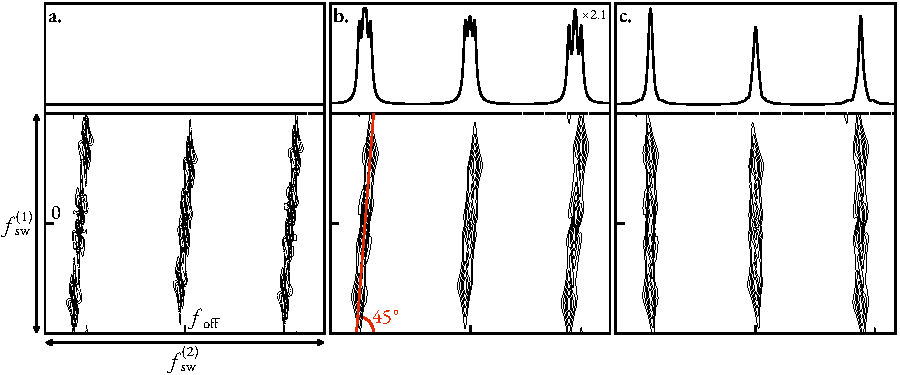
\includegraphics{jres_spectrum/jres_spectrum.pdf}%
    \caption[
        Example of a simple \acs{2DJ} spectrum derived from an AMX spin system.
    ]
    {%
        \textbf{a.} Contour plot of an absolute value mode \ac{2DJ} spectrum for an
        AMX spin system, produced by applying sine-bell apodisation on a hypercomplex
        \ac{FID} before a \ac{FT} in both dimensions. Each multiplet lies a
        long a line at \ang{45} to the $F^{(1)}$ and $F^{(2)}$ axes. Note that
        this line often appears to make an angle that is greater than \ang{45}
        with the $F^{(2)}$ axis when viewing spectra, since typically $\fswone
        \ll \fswtwo$. Above the \ac{2DJ} spectrum is a plot of its summation
        along the $\Fone$ axis.
        \textbf{b.} Spectrum generated after application of a \ang{45} shear,
        with its $\Fone$ summation above.
   }%
    \label{fig:jres_spectrum}%
\end{figure}%

An FID generated by the \ac{2DJ} experiment is hypercomplex, taking the form of
\eqref{eq:general-fid} with $D=2$ and $\zeta = \exp(\iu\cdot)$, i.e.
\begin{equation}%
    \begin{split}%
        \jresfid\idxnonentwo =
        \sum_{m=0}^{M-1} \bdam \exp\left( \iu \bdphim \right)
            \exp\left(\left(2 \pi \iu \bdfonem
            - \bdetaonem\right) {\none}_{\vphantom{t}} \Dtone\right) \times \\
            \exp\left(\left(2 \pi \iu  \left(
            \bdftwom - \fofftwo \right)
            - \bdetatwom\right) {\ntwo}_{\vphantom{t}} \Dttwo\right)
            + \symbf{W}\left[n^{(1)}, n^{(2)}\right].
    \end{split}%
    \label{eq:jres-fid}
\end{equation}%
The transmitter offset term has been neglected in the indirect dimension, since chemical shift evolution does not occur.
A major downside of the \ac{2DJ} experiment is there is no means of generating
a pair of phase- or amplitude-modulated signals which are the
conventional route to frequency-discriminated spectra with absorption mode lineshapes, as no mixing time exists in the pulse sequence. The FT of $\jresfid$ produces a spectrum
$\jresspec$ with phase-twist peaks \note{Reference chapter 1 when 2D spectrum processing has been described}, which possess contributions from both absorption
and dispersion Lorentzians.
As with other experiments which produce hypercomplex signals, such as \ac{COSY}, the data is displayed in magnitude-mode, in which the absolute value of each point in the spectrum is displayed.

There are two primary steps involved in obtaining a
pure shift spectrum from $\jresspec$:
\begin{enumerate}
    \item Perform a \ang{45} shear (often called a tilt) on the spectrum array,
        leading to the separation of chemical shifts and scalar couplings onto
        orthogonal axes  (panel b. in Figure \ref{fig:jres_spectrum}). Each
        slice in $\Ftwo$ is subjected to a right circular rotation such that
        \begin{subequations}
            \begin{gather}
                \jresspectilt\left[{\none}\vpsub{\mathrm{sw}},{\ntwo}\vpsub{\mathrm{sw}}\right] =
                \jresspec\left[{\none}\vpsub{\mathrm{sw}},\ntwonew\right],\\
                \ntwonew = \left(
                    {\ntwo}\vpsub{\mathrm{new}} + \left\lfloor
                        \frac
                            {\fswone \Ntwo\vpsub{\mathrm{sw}}}
                            {\fswtwo \None\vpsub{\mathrm{sw}}}
                        \left(
                            \frac{\None\vpsub{\mathrm{sw}}}{2} - \none
                        \right)
                    \right\rceil
                \right) \bmod \Ntwo.
            \end{gather}
        \end{subequations}
        This achieves the mapping $\jresspec\left(\fone,\ftwo\right)
        \rightarrow \jresspec\left(\fone, \ftwo - \fone\right)$.
        The effectiveness of the shear is maximised when both
        $\nicefrac{\fswtwo}{\fswone}$ and $\nicefrac{\Ntwo}{\None}$ are powers
        of 2\note{check this}.
    \item Sum the spectrum along $\Fone$:
        \begin{equation}
            \specps\idxntwo =
            \sum_{\none=0}^{\None-1} \jresspectilt\idxnonentwo.
        \end{equation}
\end{enumerate}%
If the spectrum wasn't in magnitude-mode, shearing and summing it would lead to the absorptive and dispersive
components of the spectrum cancelling each other out.
The process still leads to undesirable pure shift spectra with broad ``wings'' on
account of the presence of dispersive character. The dispersive component can
be suppressed by appropriate processing to make the FID envelope symmetric in
both dimensions, such as with sine-bell
apodisation or pseudo-echo
reshaping\cite{Bax1981}, though this results in a significant reduction in
sensitivity being incurred.
\begin{figure}
    \centering
    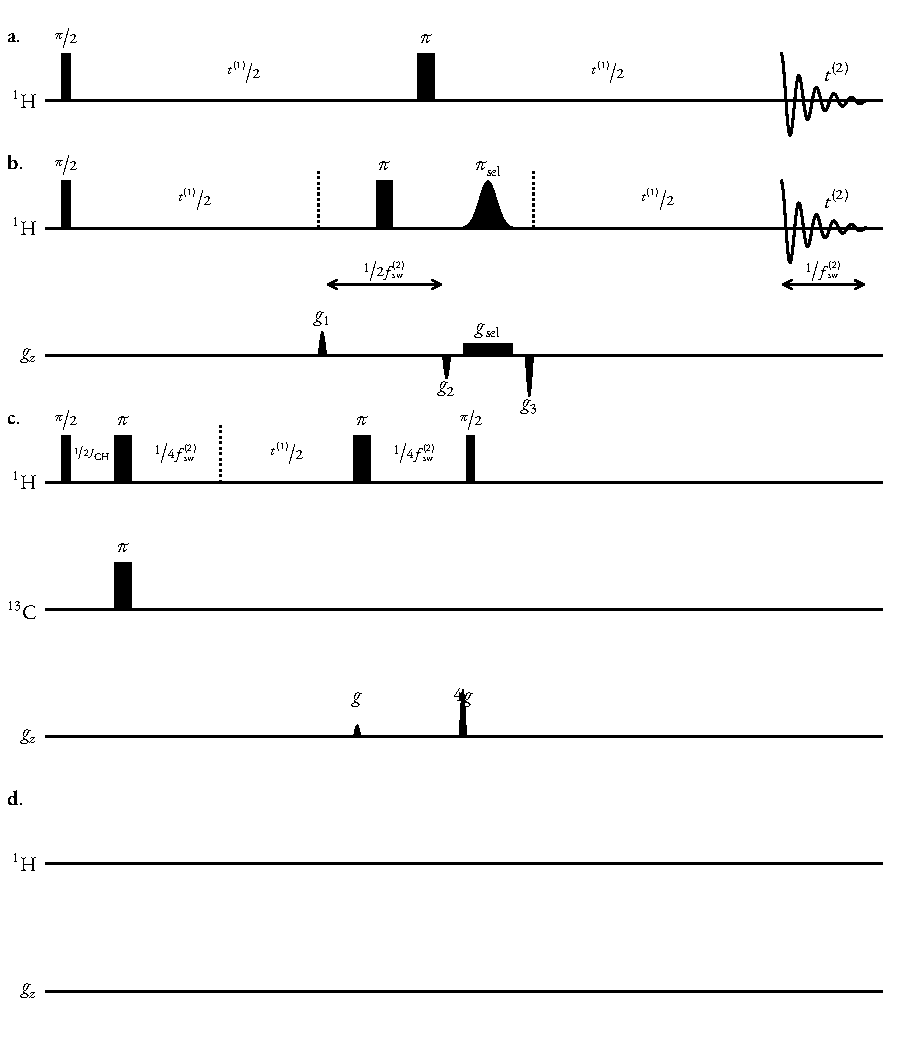
\includegraphics{pure_shift_sequences/pure_shift_sequences.pdf}
    \caption[
        The pulse sequences of some common pure shift experiments.
    ]{
        \note{Work needed. Figure out the correct delays in ZS, BIRD, PSYCHE}
        The pulse sequences of four of the most common pure shift experiments.
        \textbf{a.} \acs{2DJ}.
        \textbf{b.} The \acs{ZS} method.
        \textbf{c.} The \acs{BIRD} method.
        \textbf{d.} The \acs{PSYCHE} method.
    }
    \label{fig:pure_shift_seqs}
\end{figure}

\subsubsection{The \acl{ZS} Method}
\label{subsec:ZS}
Zangger and Sterk introduced a pulse sequence element which achieves
\emph{slice-selective excitation}, by applying a low \ac{RF} power (weak) \ang{180}
pulse\footnote{Conventionally, a R-SNOB pulse is used\cite{Kupce1995}.} in the
presence of a \ac{PFG} along the $z$-axis\cite{Zangger1997}. Such an element
excites a
given spin only in a narrow range of heights in the sample, as the \ac{PFG}
induces a shift in resonance frequency according to $\Updelta \omega(z) = \gamma
gz$, where $g$ is the magnitude of the \ac{PFG}. By placing a hard
\ang{180} pulse adjacent to the selective pulse, the
``active'' spin in a given slice is rotated by \ang{360} (i.e. no net
rotation), while all other (``passive'') spins are only rotated by \ang{180}.
Placing such a element in the middle of the $\tone$ evolution therefore
achieves refocussing of the J-couplings associated with the active
spin\cite{Aguilar2010}. In order to achieve effective decoupling of any given
pair of spins, it is necessary that the bandwidth of the selective π-pulse is
smaller than the difference in their chemical shifts. However, with more
selective pulses, a smaller proportion of the available spin magnetisation will
contribute to the final FID, and hence sensitivity will be diminished
\footnote{
    The reduction in sensitivity is $\propto \nicefrac{f_B}{\gamma G_z l_z}$,
    where $f_B$ is the selective pulse bandwidth, and $l_z$ is the length of
    the sample lying within the receiver coil ($\approx
    \qty{1.5}{\centi\meter}$).
}.
Therefore a trade-off exists between effective decoupling of all spins, and
achieving the greatest sensitivity possible. In the case of strong coupling,
the \ac{ZS} method tends to perform poorly relative to other options for this
reason. The \ac{ZS} element has been applied by Keeler and Pell in order to
generate \ac{2DJ} datasets comprising phase-modulated pairs, enabling the
generation of pure absorption-mode spectra\cite{Pell2007}, though such spectra suffer from poorer sensitivity than the conventional ``full sensitivity'' analogue.

\subsubsection{The \acs{BIRD} Method}
The \ac{BIRD} pulse sequence element\cite{Garbow1982,Bax1983}, presented in
Figure \ref{fig:pure_shift_seqs}.c, also takes advantage of the idea of
selectively inverting passive spins, while leaving active spins unaffected.
However the active spins are those which are directly bound to
\textsuperscript{13}C nuclei, which naturally occur with an abundance of 1.1\%,
while the passive spins are those bound to far more abundant
\textsuperscript{12}C nuclei. The reduction in sensitivity of the experiment
relative to a full-sensitivity experiment is therefore known and constant
across samples. In scenarios where is this strong coupling, \ac{BIRD} can
achieve improved sensitivity over \ac{ZS}, since with the latter a very weak
selective pulse would be required to ensure it is of a sufficiently small
bandwidth. The \ac{BIRD} method is particularly attractive in scenarios where
the sensitivity penalty due to the involvement of a low-abundance nucleus has
already been paid, for example in sequences where an \ac{INEPT} block is present.

\subsubsection{PSYCHE}
\label{subsec:psyche}
\note{TODO}
Original paper\cite{Foroozandeh2014}, tutorial paper\cite{Foroozandeh2018}, PSYCHE-2DJ\cite{Kiraly2017}.

\subsubsection{Pure Shift NMR via J-Resolved Post-Processing}

There have been previous descriptions of acquiring pure-shift spectra from
conventional \ac{2DJ} datasets via more sophisticated post-processing methods.
Nuzillard introduced \ac{ALPESTRE}\cite{Nuzillard1996,Martinez2012}, in which
the parameters of each indirect-dimension FID are estimated using \ac{LPSVD},
such that there is a set of parameters $\symbf{\Theta} \in \mathbb{R}^{\Ntwo
\times 4M}$ with
\begin{equation}
    \symbf{\Theta}\left[\ntwo\right] =
    \begin{bmatrix}
        \left[\bda_{\ntwo}\right]\T &
        \left[\bdphi_{\ntwo}\right]\T &
        \left[\bdfone_{\ntwo}\right]\T &
        \left[\bdetaone_{\ntwo}\right]\T
    \end{bmatrix}\T.
\end{equation}
The parameters generated are used to propagate each FID backward into
$-\tone$, producing a ``full-echo'':
\begin{equation}
    \begin{split}
        \symbf{Y}_{\text{full}}\left[\none, \ntwo\right] = \sum_{m=0}^{M-1}
            \bda_{\ntwo} \left[ m \right]
            \exp\left(\iu \bdphi_{\ntwo} \left[ m \right] \right)
            \exp\left(\left(2 \pi \iu \bdfone_{\ntwo} \left[ m \right] \none
            -\bdetaone_{\ntwo} \left[ m \right] \left\lvert \none \right\rvert \right)\Dtone\right), \\
        \forall \none \in \lbrace -\None + 1, \cdots, 0, \cdots, \None - 1 \rbrace,\ \forall \ntwo \lbrace 0, \cdots \Ntwo - 1 \rbrace.
    \end{split}
    \label{eq:full-echo}
\end{equation}
\ac{FT} of \eqref{eq:full-echo} generates a spectrum whose real component comprises absorption-mode
Lorentzian character in both dimensions. This opens up the means of producing
pure-shift spectra from the \ac{2DJ} experiment with sharp lineshapes and
without sensitivity loss. A similar approach proposed by Mutzenhardt et al.
instead constructed full echoes via \ac{LP} of each direct-dimension
\ac{FID}, and generation of a full echo by propagating
into $-\ttwo$\cite{Mutzenhardt1999}.

\subsection{An outline of \acs{CUPID}}
\acf{CUPID} aims to generate pure shift spectra by utilising the result of
parametric estimation of \ac{2DJ} data, assumed to take the functional form of
\eqref{eq:jres-fid}.
Instead of estimating successive \ac{1D} \acp{FID}, as has been described by
Nuzillard and Mutzenhardt et al., the entire \ac{2DJ} signal is estimated as a
whole, giving access to the parameter vector $\bth \in \mathbb{R}^{6M}$. With knowledge of the frequencies and damping factors in both dimensions, it is possible to generate \iac{FID} which will produce a pure shift spectrum directly, rather than constructing a full-echo \ac{2DJ} signal, and subsequently shearing and summing it. The desired signal is named
the ``\ang{-45} signal'' (Figure
\ref{fig:neg-45}), and has the form:
\begin{equation}
    \begin{split}
        \symbf{y}_{\ang{-45}}\left(\bth\right)\left[ \ntwo \right] =
            \sum_{m=0}^{M-1} \bdam \exp \left(\iu \bdphim \right)\\
            \exp\left(
                \left(
                    2 \pi \iu \left(\bdftwom - \bdfonem - \fofftwo\right)
                    - \bdetatwom
                \right) \ntwo \Dttwo
            \right)
    \end{split}
    \label{eq:neg-45}
\end{equation}
$\forall \ntwo \in \lbrace 0, \cdots, \Ntwo - 1 \rbrace$. The \ang{-45} signal
takes the same functional form as a typical \ac{1D}
\ac{FID} acquired by a pulse-acquire experiment, except that the frequency of
each oscillator, which would usually be $\ftwo$, is replaced with $\ftwo -
\fone$. In a \ac{2DJ} experiment, $\fone$ corresponds to the displacement of a
given oscillator from the central frequency of the multiplet it is associated
with. As such, the oscillators belonging to a given multiplet all provide
a contribution with the same frequency to the \ang{-45} signal, namely the
chemical shift of the relevant spin.
\begin{figure}
    \centering
    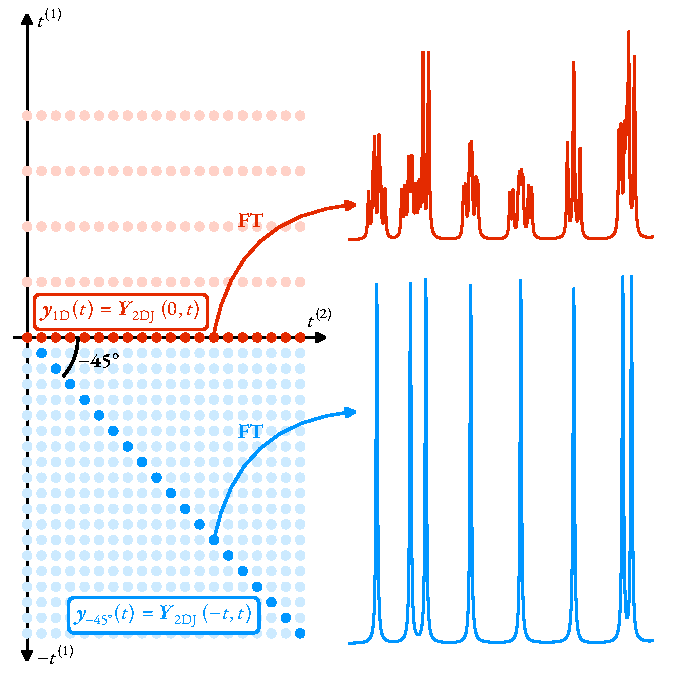
\includegraphics{neg_45_signal/neg_45_signal.pdf}
    \caption[
        An illustration of the reasoning behind the name ``\ang{-45}
        signal''.
    ]{
        An illustration of the reasoning behind the name ``\ang{-45}
        signal''. The pale red dots denote a typical \ac{2DJ} \ac{FID}, where
        the amount and rate of sampling in the direct dimension is greater than
        in the indirect dimension (i.e. $\None \ll \Ntwo$ and $\fswone \ll
        \fswtwo$). The bright red dots correspond to the first direct-dimension
        signal $\bY_{\text{2DJ}}(0, \ttwo)$, which has the same form as
        \iac{FID} from a pulse-acquire experiment. A hypothetical signal
        generated by propagating the \ac{FID} into $-\tone$, with the same rate
        of sampling in both dimensions, is denoted with pale blue dots. Taking
        the diagonal of this signal, such that it forms a \ang{-45} angle to the
        $\ttwo$ axis, yields an \ac{FID} $\by_{\ang{-45}}$  which is
        homodecoupled. Note that there is a slight discrepancy
        between \eqref{eq:neg-45} and this description, in that the
        indirect-dimension damping factors $\bdetaone$ are neglected in the
        former case.
    }
    \label{fig:neg-45}
\end{figure}

\subsubsection{Multiplet Prediction}
A holistic \ac{2D} estimation of the \ac{FID} provides access to other useful
information about the dataset. One such example is the grouping of oscillators
on account of which multiplet structure they belong to. As has already been
established, for oscillators which are associated with the same multiplet
structure, the quantity $\ftwo - \fone$ should be equal. This provides a
criterion in order to assess whether it is likely that two oscillators in the
estimation result belong to the same multiplet:
\begin{equation}
    \left \lvert
        \left( \bdftwo \left[ m_1 \right] -
        \bdfone \left[ m_1 \right] \right) -
        \left( \bdftwo \left[ m_2 \right] -
        \bdfone \left[ m_2 \right] \right)
    \right \rvert < \epsilon
\end{equation}
$\forall m_1, m_2 \in \lbrace 0, \cdots, M-1 \rbrace$, with  $\epsilon \in
\mathbb{R}_{>0}$ being a suitable threshold to account for error in the
estimation. An appropriate value for $\epsilon$ is the
spectral resolution in the more poorly resolved dimension, i.e.
$\epsilon = \min\left(\nicefrac{\fswone}{\None}, \nicefrac{\fswtwo}{\Ntwo}\right)$. In situations involving real \ac{2DJ}
signals however, it is found that $\epsilon$ sometimes has to be increased to
values slightly larger than this to achieve effective groupings (\textit{vide
infra}). Algorithm \ref{alg:mp-assign} provides a routine that can be used for
multiplet prediction.

The ability to predict multiplet groupings can also assist in scenarios where the estimation result contains some oscillators with a spurious nature, typically due to overfitting. These typically possess either a very large damping factor or low amplitude, and are not associated with discernible peaks
in the spectrum. Part of the reason that the variance of phases is included in
the fidelity for \ac{NLP} is to try and purge these oscillators,
however this method is not infallible, and undesired oscillators can end up in
the final result. An appreciable number of these can be removed in an automated
fashion by noting that there should not be any oscillators in the estimation
result of a 2DJ dataset which satisfy both of the following:
\begin{enumerate}
    \item The oscillator is not grouped with any other oscillator as part of
        the multiplet assignment.
    \item The magnitude of the indirect dimension frequency of the oscillator
        is appreciably greater than \qty{0}{\hertz}.
\end{enumerate}
These criteria are borne out of the fact that it should not be possible to have
oscillators in a 2DJ dataset which are not part of a multiplet structure,
unless such oscillators are singlets. As no scalar couplings contribute, these
singlets should have an indirect dimension frequency of \qty{0}{\hertz}.

\subsubsection{Filtration of \ac{2DJ} data}
Unlike the direct-dimension, which can often comprise sparsely distributed
peaks in the Fourier domain, the indirect dimension of \ac{2DJ} datasets tends
to be rather densely populated. As such, it is typically of little use in
attempting to generate filtered sub-\acp{FID} in the indirect dimension. The
filtering procedure utilised for \ac{2DJ} data is therefore an extension of the
filtration procedure for \ac{1D} data described in Section \ref{sec:filtering}
(Figure \ref{fig:jres-filtering}). The filtering procedure involves the
following steps:
\begin{enumerate}
    \item The signal $\symbf{Y}_{\text{ve}} \in \mathbb{C}^{\None \times 2 \Ntwo}$ is
    constructed, such that a virtual echo is formed from each direct-dimension
    signal:
    \begin{equation}
        \begin{split}
            \symbf{Y}_{\text{ve}} \left[n^{(1)}\right] =
                &\left[
                \begin{matrix}
                    \Re\left(\symbf{Y}\left[n^{(1)}, 0\right]\right) &
                    \symbf{Y}\left[n^{(1)}, 1\right] &
                    \cdots
                \end{matrix}\right.
                \\
                &\left.
                \begin{matrix}
                    \symbf{Y}\left[n^{(1)}, \Ntwo - 1\right] &
                    0 &
                    \symbf{Y}\left[n^{(1)}, \Ntwo - 1\right]^* &
                    \cdots &
                    \symbf{Y}\left[n^{(1)}, 1\right]^*
                \end{matrix}
                \right]
        \end{split}
    \end{equation}
    $\forall n^{(1)} \in \lbrace 0, \cdots, N^{(1)} - 1 \rbrace$.
    \item $\symbf{Y}_{\text{ve}}$ is subjected to \ac{FT} along the direct
        dimension to produce the spectrum  $\symbf{S}_{\text{ve}}$ (panel a of
        Figure \ref{fig:jres-filtering}). This has a imaginary component of
        zeros.
    \item A super-Gaussian $\symbf{G} \in \mathbb{R}^{\None \times 2 \Ntwo}$ is
        constructed (panel b):
        \begin{equation}
            \symbf{G} = \symbf{1} \otimes \symbf{g}^{(2)},
        \end{equation}
        where $\symbf{1} \in \mathbb{R}^{\None}$ is a vector of ones, and
        $\symbf{g}^{(2)}$ is a super-Gaussian vector given by
        \eqref{eq:super-Gaussian-onedim} with $d=2$.
    \item A matrix of additive noise is generated by extracting the variance
        $\sigma^2$ of a strip of $\symbf{S}_{\text{ve}}$ which is devoid of
        peaks, and generating an array $\symbf{W}_{\sigma^2} \in
        \mathbb{R}^{\None \times 2 \Ntwo}$ with values independently sampled
        from a normal distribution with mean $0$ and variance  $\sigma^2$.
    \item The spectrum is filtered according to \eqref{eq:Sve-tilde}, yielding
        $\widetilde{\symbf{S}}_{\text{ve}}$ (panel d).
    \item $\widetilde{\symbf{S}}_{\text{ve}}$ is subjected to \ac{IFT} and is
        sliced in half in the direct dimension, yeilding the final filtered
        signal $\widetilde{\symbf{Y}}$:
        \begin{equation}
            \widetilde{\symbf{Y}} = \IFT^{(2)}\left(\widetilde{\symbf{S}}_{\text{ve}}\right) \left[:, : \Ntwo\right].
        \end{equation}
\end{enumerate}

\begin{figure}
    \centering
    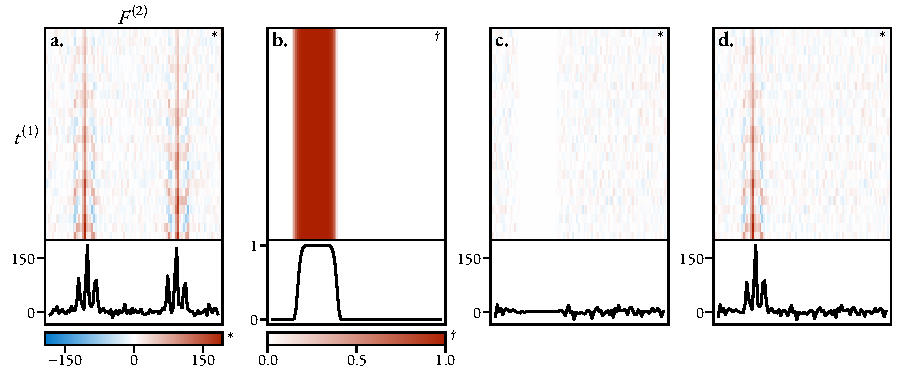
\includegraphics{jres_filtering/jres_filtering.pdf}
    \caption[
        An illustration of the filtering procedure for \ac{2DJ} data.
    ]
    {
        An illustration of the filtering procedure for \ac{2DJ} data.
        For each panel is a heat-map of the full \ac{2D} signal, as well as a
        plot underneath of the first slice of the signal in the direct
        dimension.
        \textbf{a.} The spectrum $\symbf{S}_{\text{ve}}$,
        \textbf{b.} Super-Gaussian filter $\symbf{G}$,
        \textbf{c.} Additive noise, attenuated by the super-Gaussian, $\symbf{W}_{\sigma^2} \odot (\symbf{1} - \symbf{G})$,
        \textbf{d.} Filtered spectrum $\widetilde{\symbf{S}}_{\text{ve}}$
        Panels \textbf{a.}--\textbf{d.} are analogous to panels \textbf{b.}--
        \textbf{e.} in Figure \ref{fig:filtering} for the \ac{1D} case.
    }
    \label{fig:jres-filtering}
\end{figure}

\subsection{Results Using \acs{CUPID}}
\label{subsec:cupid-results}
A number of examples of the application of \ac{CUPID} are now provided.
Initially, a few results are presented using data simulated using the Spinach
MATLAB\textregistered\ library\cite{Hogben2011}.
After this, examples are provided with experimental data. In a couple of these,
comparison of the result acquired using \ac{CUPID} is compared with a spectrum
acquired using \ac{PSYCHE}.

For additional details relating to generation of the simulated datasets, see
section \ref{sec:simulated-datasets} in the Appendix.

\subsubsection{``Four Multiplets''}
\begin{figure}
    \centering
    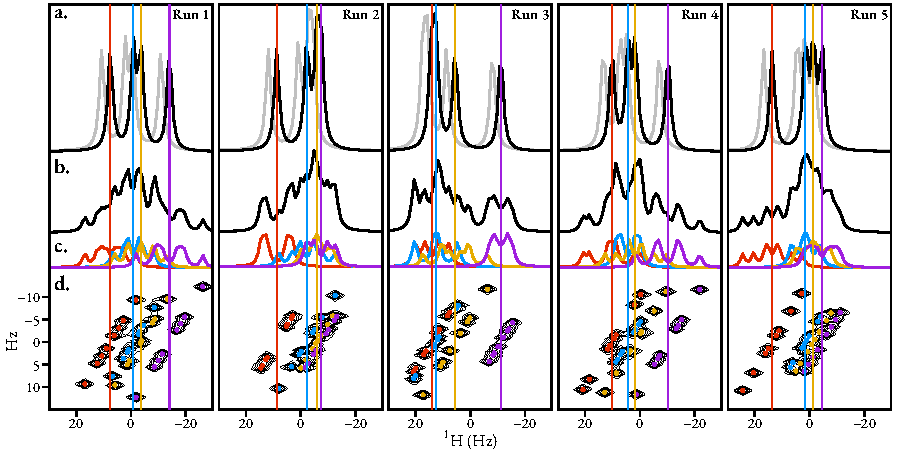
\includegraphics{four_multiplets/four_multiplets}
    \caption[
        The result of applying \acs{CUPID} to 5 instances of simulated
        \acs{2DJ} datasets with 4 heavily overlapping multiplet structures.
    ]{
        The result of applying \ac{CUPID} to 5 instances of simulated \ac{2DJ}
        datasets with 4 heavily overlapping multiplet structures.
        \textbf{a.} Black: pure shift spectrum generated by \ac{CUPID}.
        Grey: \ac{1D} spectrum simulated with Spinach, using the same spin
        system as was used to produce the \ac{2DJ} dataset, but with all scalar
        couplings sets to \qty{0}{\hertz}. This has been offset slightly for
        clarity.
        \textbf{b.} \ac{1D} spectrum of the dataset.
        \textbf{c.} Multiplet structures predicted, using a threshold $\epsilon
        = \nicefrac{\fswtwo}{\Ntwo} \approx \qty{0.98}{\hertz}$.
        \textbf{d.} Contour plot of the \ac{2DJ} spectrum in absolute-value
        mode. Coloured points denote the frequencies of oscillators in the
        estimation result.
        Coloured vertical lines denote the predicted central frequencies of
        each multiplet structure.
    }
    \label{fig:four-multiplets}
\end{figure}
A series of simulated \proton\ \ac{2DJ} datasets were generated such that
within a known region of the spectrum, four ddd multiplet structures with
significant overlap existed. To achieve this, a spin-system with 7 spins was
formed, with the spins divided into 2 subsets:
\begin{itemize}
    \item 4 of the spins (the ``estimated spins'') were assigned random
        resonance frequencies sampled from $\mathcal{U}(\qty{-20}{\hertz},
        \qty{20}{\hertz})$.
    \item The remaining 3 spins (the ``coupling spins''), were coupled to each
        of the estimated spins, with the values of the couplings randomly
        sampled from $\mathcal{U}(\qty{-10}{\hertz}, \qty{10}{\hertz})$.  The
        coupling spins were given chemical shifts such that they lay far from
        the estimated spins in the spectrum (i.e. their frequencies were $\gg
        \qty{20}{\hertz}$).
\end{itemize}
\ac{AWGN} noise was added to the \ac{FID}, with a target \ac{SNR} of \qty{30}{\deci\bel}.
A filtered sub-\ac{FID} containing only the signals from the estimated spins
was then generated using the filtering procedure described above, with
$l^{(2)}_{\unit{\hertz}} = \qty{30}{\hertz}$,
$r^{(2)}_{\unit{\hertz}} = \qty{-30}{\hertz}$.
The resulting sub-\ac{FID} was expected to comprise 32 ($4 \times
2^3$) oscillators. To assess the estimation procedure's ability, a random
integer from the range 33 -- 40 was selected as the initial number of
oscillators. Hence, the initial guess from the \ac{MMEMPM} would comprise an
excessive number of oscillators. The \ac{FID} was subjected to
estimation, yielding the result vector $\bthstar$. Spurious oscillators were
checked for, using the criteria outlined above, with the threshold for
multiplet assignment set to the spectral resolution in the direct
dimension:
$\epsilon = \nicefrac{f_{\text{sw}}^{(2)}}{\Ntwo}$.  If spurious oscillators
were found, these were removed, and \ac{NLP} was run on the updated set of
parameters.

Figure \ref{fig:four-multiplets} illustrates the result achieved for 5 separate
runs of this procedure.
For each \ac{FID} generated, the method was effective at producing an
estimation result with 32 oscillators, as desired, despite the excessive number
that were present in $\bthzero$. Most of the excessive oscillators were purged
from $\bthzero$ through the \ac{NLP} procedure. When spurious oscillators did
remain\footnote{for 2 of the 5 datasets, the result after \ac{NLP} comprised 33
oscillators}, they were then detected when checking for spurious oscillators
and subsequently removed. The pure-shift spectra generated using \ac{CUPID}
closely agree with pure-shift spectra generated by running a Spinach simulation
on a spin system with the same chemical shifts, but with all scalar couplings
set to \qty{0}{\hertz}.

\subsubsection{``Sucrose''}
\begin{figure}
    \centering
    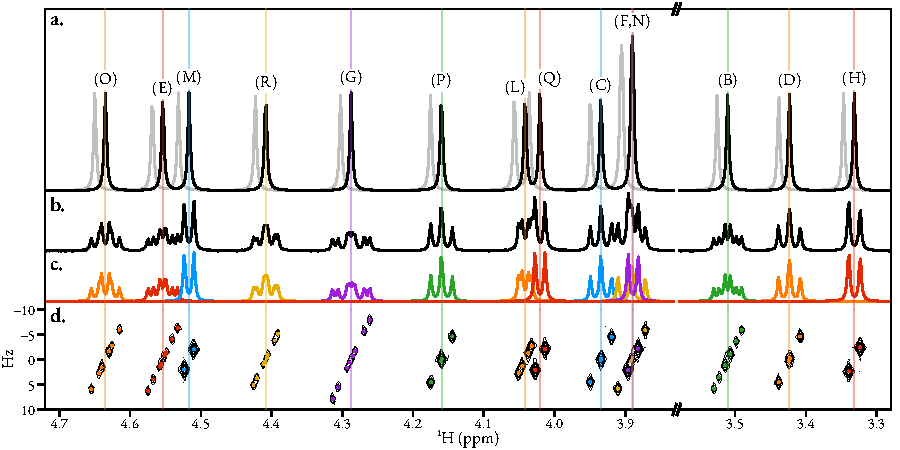
\includegraphics{sucrose_cupid/sucrose_cupid.pdf}
    \caption[
        Application of \acs{CUPID} on a simulated sucrose \acs{2DJ} dataset.
    ]
    {
        Application of \ac{CUPID} on a simulated sucrose \ac{2DJ} dataset.
        \textbf{a.} Black: the spectrum generated from \ac{FT} of the \ang{-45}
        signal. Grey: the spectrum of a simulated dataset with the same
        chemical shifts, with all scalar couplings set to \qty{0}{\hertz}.
        \textbf{b.} Conventional \ac{1D} spectrum.
        \textbf{c.} Multiplet structures assigned ($\epsilon \approx
        \qty{0.27}{\hertz}$).
        \textbf{d.} Contour plot of the absolute value mode \ac{2DJ} spectrum,
        with the locations of assigned oscillators given as coloured points.
    }
    \label{fig:sucrose-cupid}
\end{figure}
As a second example of applying \ac{CUPID} on simulated data, the chemical
shifts and isotropic scalar couplings associated with a
Gaussian\cite{Gaussian03} \ac{DFT} calculation of sucrose in a vacuum
\footnote{
It is well known that isotropic chemical shift calculations using \ac{DFT} are
typically very inaccurate. The resulting spectrum is not typical of sucrose in
the liquid state, though this doesn't really matter for assessing the
performance of \ac{CUPID}.
}
were used to construct a 2DJ dataset. \ac{AWGN} was added with a target
\ac{SNR} of \qty{20}{\deci\bel}. The CUPID procedure was applied to filtered
sub-FIDs such that the resonances from all 22 spins were considered, though
only the regions of the dataset with the most interesting multiplet structures
are presented in Figure \ref{fig:sucrose-cupid}.

The estimation technique successfully assigned multiplet structures for all 22
multiplets in the dataset, including structures derived from two spins (F \& N)
with a \qty{0.6}{\hertz} difference in resonance frequency, approaching the
spectral resolution in the direct dimension (\qty{0.537}{\hertz}). The
pure-shift spectrum generated via the \ang{-45} signal again showed close
agreement with a 1D spectrum simulated using the same chemical shifts, with
scalar couplings set to \qty{0}{\hertz}. There are particular multiplets where
the number of oscillators fit using the estimation routine was less than the
true number. Examples of this phenomenon are exhibited in the estimates of the
multiplets for spins B \& O, which are both ddd structures. The scalar
couplings involved meant that certain oscillators were
of such similar frequencies that they were separated by significantly less than
the spectral resolution, and thus resolving these was unrealistic. For
example, there are two pairs of peaks in the spin-B multiplet which lie only
\qty{0.085}{\hertz} apart. Under-fitting in this case had a negligible impact
on the final pure shift spectrum. However there are circumstances which will be
seen in the experimental examples below where more blatant cases of under-fitting
lead to the generation of peaks in the pure shift spectrum which are noticeably
broadened.

\subsubsection{Quinine}
\begin{figure}
    \centering
    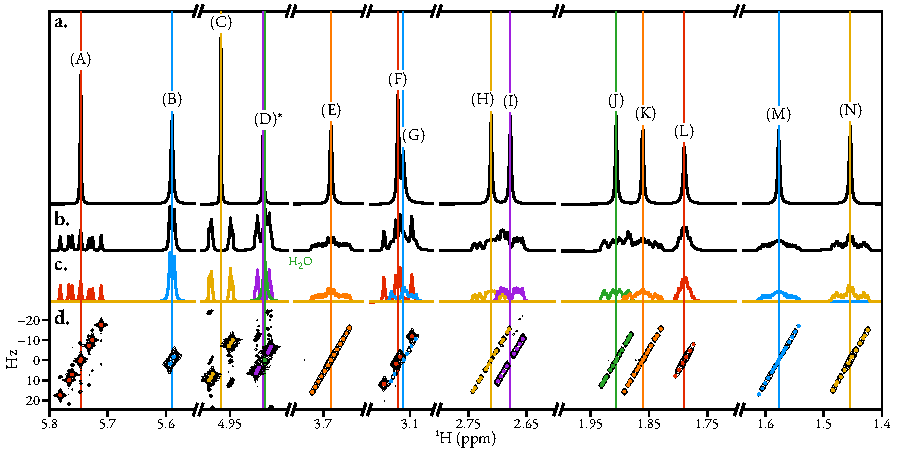
\includegraphics{quinine_cupid/quinine_cupid.pdf}
    \caption[
        Application of \acs{CUPID} on the non-aromatic regions of a quinine
        \acs{2DJ} dataset.
    ]{
        Application of \ac{CUPID} on the non-aromatic regions of a quinine
        \ac{2DJ} dataset.
        \textbf{a.} The spectrum generated from \ac{FT} of the \ang{-45}
        signal, with the green signal arising from water at about
        \qty{4.89}{\partspermillion} neglected.
        \textbf{b.} Conventional \ac{1D} spectrum.
        \textbf{c.} Multiplet structures assigned ($\epsilon =
        \nicefrac{\fswtwo}{\Ntwo} \approx \qty{0.92}{\hertz}$).
        \textbf{d.} Contour plot of the absolute value mode \ac{2DJ} spectrum,
        with the locations of assigned oscillators given as coloured points.
    }
    \label{fig:quinine-cupid}
\end{figure}

Figure \ref{fig:quinine-cupid} illustrates the result of applying \ac{CUPID} on
a dataset generated from a sample comprising quinine in CD\textsubscript{3}OD,
with all non-aromatic protons considered. The method successfully generated a
pure shift spectrum with distinct peaks for each \textsuperscript{1}H
environment. This example also highlights an added benefit of using \ac{CUPID}:
the ability to suppress unwanted signals in the pure shift spectrum. In this
example, an intense, broad singlet at around \qty{4.89}{\partspermillion}
was detected (see the green peak at this frequency in panel c).
The singlet was due to the presence of water in the sample and was a hindrance
due to it overlapping heavily with the multiplet structure corresponding to
spin D. To obtain a clean singlet for spin D in the pure shift spectrum, the
oscillator corresponding to the water signal was simply neglected from
the parameter set used to
generate the \ang{-45} signal. \note{Find reference for work
talking about using estimation for solvent suppression.}

As eluded to already, a few of the peaks in the pure-shift spectrum are rather
broad on account of the estimation routine under-fitting the relevant multiplet
structure. The most notable example of this phenomenon in the quinine example
comes from the peak for spin G, where significant overlap with spin F has likely
compounded the task of accurately estimating the relevant oscillators \ac{FID}. With fewer than the
true number of oscillators fitting a given multiplet structure, the \ac{NLP}
routine will compensate by giving the oscillators it does have at its disposal
large amplitudes and damping factors, so that they can reasonably fit multiple
similar-frequency oscillators.
While affecting peak linewdiths, this feature does not tend to significantly
affect the integrals of the pure shift peaks. \note{Should probably calculate
the integrals of these...}

\subsubsection{Camphor}
\begin{figure}%
    \centering%
    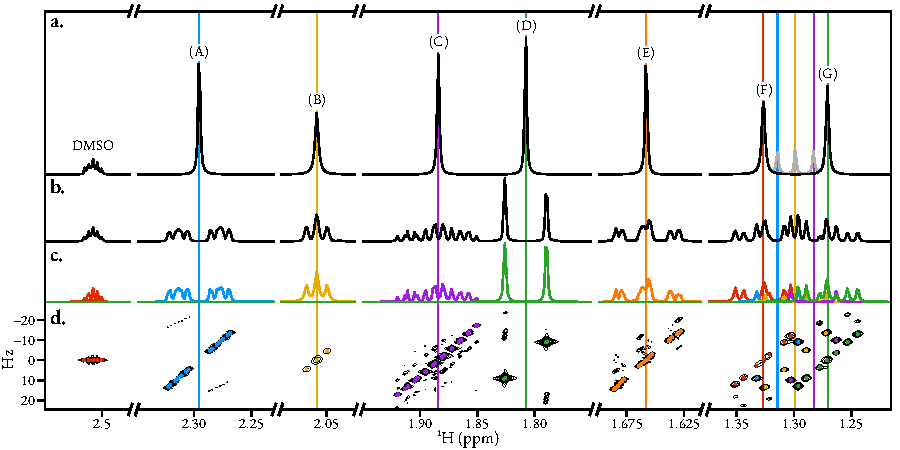
\includegraphics{camphor_cupid/camphor_cupid.pdf}%
    \caption[
        Application of \acs{CUPID} on a camphor dataset.
    ]{
        Application of \acs{CUPID} on camphor \ac{2DJ} dataset.
        \textbf{a.} Black: the spectrum generated from \ac{FT} of the \ang{-45}
        signal. Oscillators associated with strong coupling artefacts between
        spins (F) and (G) were neglected. Grey: spectrum generated without
        neglecting oscillators associated with strong coupling artefacts.
        \textbf{b.} \acs{1D} spectrum produced from the first direct-dimension
        \ac{FID} in the dataset. Note that, unlike a conventional pulse-acquire
        spectrum, strong coupling artefacts are present.
        \textbf{c.} Multiplet structures assigned ($\epsilon =
        \nicefrac{2 \fswtwo}{\Ntwo} \approx \qty{1.23}{\hertz}$).
        \textbf{d.} Contour plot of the absolute value mode \acs{2DJ} spectrum,
        with the locations of assigned oscillators given as coloured points.
    }
    \label{fig:camphor-cupid}%
\end{figure}%
The application of \ac{CUPID} to the non-methyl regions of a \ac{2DJ}
dataset of camphor (Figure \ref{fig:structures}.c) in \acs{DMSOd6} is presented
in Figure \ref{fig:camphor-cupid}. As in the quinine case, there are instances
of underfitting, which lead to broadening of the resulting pure shift peak,
with the peak associated with spin (B) being the most drastic example of this.
This example highlights the ability of \ac{CUPID} to remove undesirable
\emph{strong coupling artefacts}\footnote{
    As stressed in \cite{Thrippleton2005}, these are not strictly artefacts,
    but rather genuine signals, which are expected to be present in the
    \ac{2DJ} dataset. Despite this, the term is widespread in the literature.
}from the final pure shift spectrum, which
arise due to mixing effects induced by the \ang{180} pulse in the \ac{2DJ}
sequence\cite{Thrippleton2005,Wider1983}.
The effects of strong coupling lead to the presence of extra unexpected peaks
which do not agree with the chemical shift of any spin associated with camphor.
Such effects are observed between roughly \SIrange{1.35}{1.25}{\partspermillion} in
the camphor spectrum, where artefacts associated with spins (F) and (G) exist.
The estimation routine was able to determine parameters for
the more intense oscillators which make up the strong coupling artefacts (these
are coloured blue, yellow, and purple, while oscillators associated with the
true multiplet structures for (F) and (G) are coloured red and green, respectively).
Inclusion of all oscillators extracted by the estimation routine generates the
spectrum in panel a, with the low-intensity grey peaks associated with the strong
coupling effects included. However, in much the same way as the water signal in
the quinine example could be neglected, it is trivial to construct the \ang{-45}
signal with the oscillators associated with strong coupling neglected, which
produces the black spectrum.

\subsubsection{Dexamethasone}

\begin{sidewaysfigure}%
    \centering%
    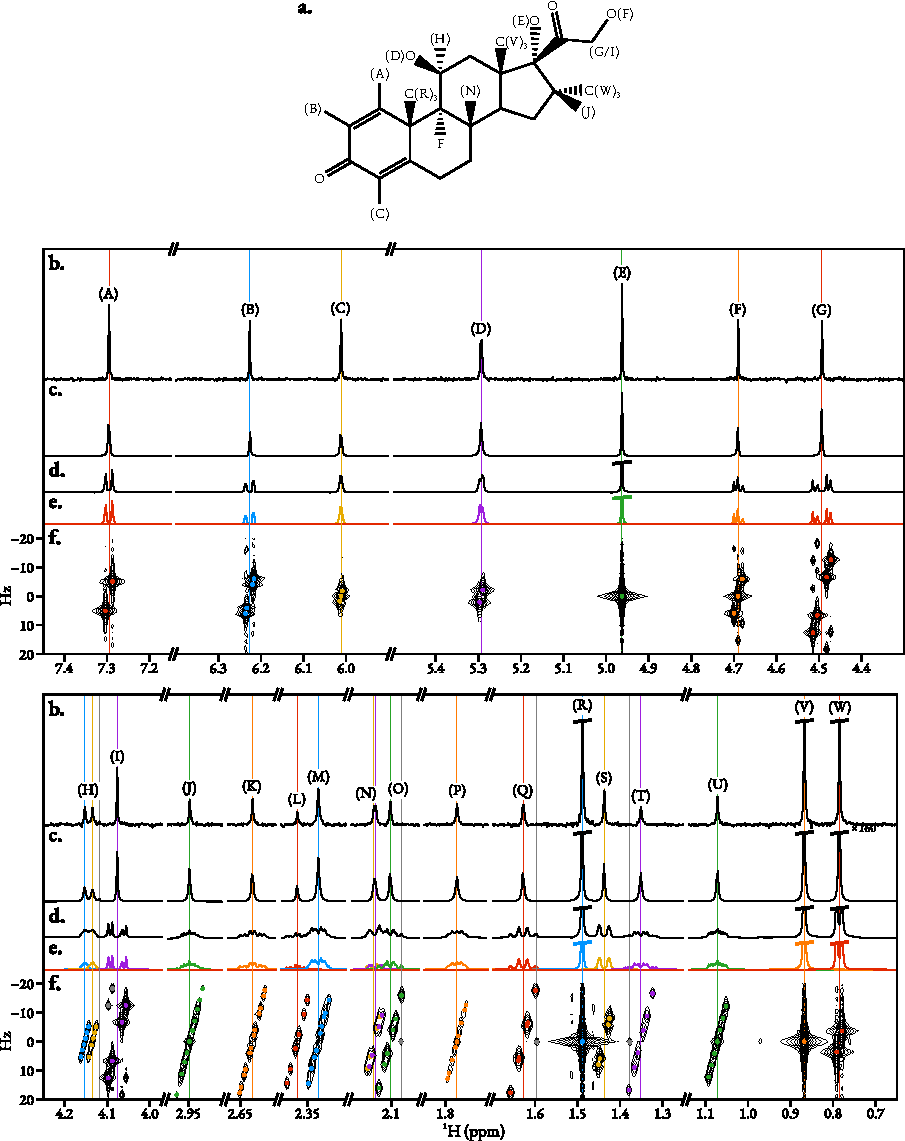
\includegraphics{dexamethasone_cupid/dexamethasone_cupid.pdf}%
    \caption[
        Application of \acs{CUPID} on a dexamethasone dataset.
    ]{
        \note{Fix magnification label.}
        Application of \acs{CUPID} on dexamethasone \ac{2DJ} dataset.
        \textbf{a.} \acs{TSE-PSYCHE} spectrum of the sample.
        \textbf{b.} The spectrum generated from \ac{FT} of the \ang{-45}
        signal.
        \textbf{c.} Conventional \acs{1D} spectrum.
        \textbf{.} Multiplet structures assigned ($\epsilon =
        \nicefrac{\fswtwo}{\Ntwo} \approx \qty{0.92}{\hertz}$).
        \textbf{d.} Contour plot of the absolute value mode \acs{2DJ} spectrum,
        with the locations of assigned oscillators given as coloured points.
    }
    \label{fig:dexamethasone-cupid}%
\end{sidewaysfigure}%
\note{Double check mp thold}

Figure \ref{fig:dexamethasone-cupid} shows the result of applying CUPID on a
dataset acquired from a sample dexamethasone in DMSO-d\textsubscript{6}. A
pure-shift spectrum was also acquired using the
\ac{TSE-PSYCHE} experiment\cite{Foroozandeh2018,Foroozandeh2015} for
comparison.
\ac{CUPID} generated a pure-shift spectrum with overall excellent agreement
with the \ac{TSE-PSYCHE} spectrum. Certain multiplet structures in the spectrum exhibit
splitting in $\Ftwo$, on account of heteronuclear couplings to \textsuperscript{19}F. Most
notable are those derived from spins (D), (H) \& (O). For the (D) multiplet, the
magnitude of the heterocoupling is very small such that assigning these to
separate oscillators is infeasible.
For the spin (N) multiplet, two separate structures were successfully assigned
(see the orange and green multiplets around \qty{2.1}{\partspermillion}).
The estimation routine was unsuccessful at accurately estimating the structure
associated with spin (H), where a severe under-fitting occurred. An under-fitting
of this structure even occurred when the estimation was re-run using
considerable over-estimation of the model order, with most oscillators in the
initial guess being purged during the \ac{NLP} procedure.
The spin (H) multiplet provides an extreme example line-broadening in the pure
shift spectrum on account of under-fitting. The most downfield peaks in the
CUPID spectrum (corresponding to aromatic and hydroxyl protons) also appear to
be noticeably broadened relative to their PSYCHE equivalents. This is also
probably due to under-fitting of the relevant multiplet structures, though to a
far less noticeable extent than for spin H. \note{Any other reason why this
might be so?}

\subsubsection{Estradiol}
\begin{figure}
    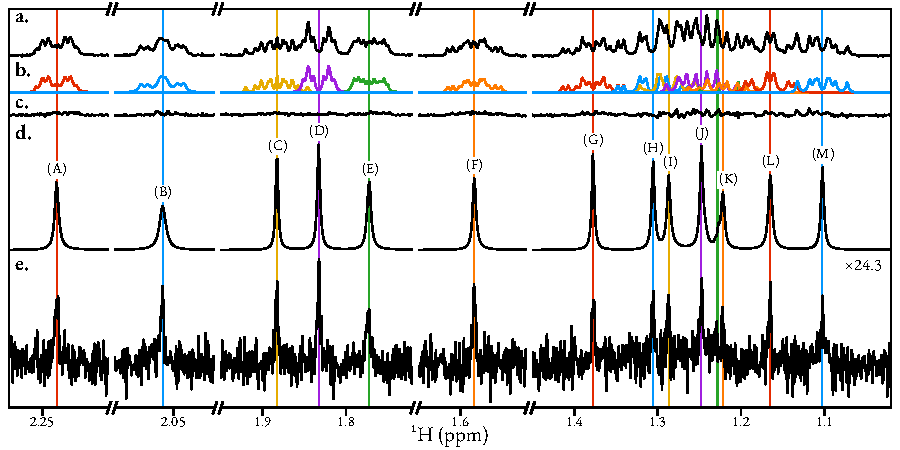
\includegraphics{estradiol_cupid/estradiol_cupid.pdf}%
    \caption[
        Application of \acs{CUPID} on a 17\textbeta-estradiol dataset.
    ]{
        Application of \acs{CUPID} on \ac{2DJ} dataset of 17\textbeta-estradiol
        in \acs{DMSOd6}.
        \textbf{a.} Spectrum of the first direct-dimension \ac{FID} in the
        \ac{2DJ} dataset.
        \textbf{b.} Multiplet structures assigned ($\epsilon =
        \nicefrac{\fswtwo}{\Ntwo} \approx \qty{2}{\hertz}$).
        \textbf{c.} The residual between the spectrum in panel a and the lines
        in panel b.
        \textbf{d.} The pure shift spectrum generated using \ac{CUPID}.
        \textbf{e.} \acs{PSYCHE} spectrum of the sample see Figure
        \ref{fig:psyche} for details on the pulse sequence. The spectrum has
        been scaled such that the maximum is of the same magnitude as the
        corresponding point in the \ac{CUPID} spectrum.
    }
    \label{fig:estradiol-cupid}%
\end{figure}

A final showcase of \ac{CUPID} is provided by Figure \ref{fig:estradiol-cupid}, where a low concentration (\qty{2}{\milli\molar}) sample of 17\textbeta-estradiol (Figure \ref{fig:structures}.
